\chapter{Notable Results}
In this chapter I will present specifics of my two best models, once the Vanilla U-Net that has reached the best IoU scores during Overfitting and once the Attention U-Net that was explored in the last phase of the project (Section \ref{sec:squeeze_the_juice} "Squeeze The Juice").

\section{Vanilla U-Net}
The Vanilla U-Net with \texttt{128} base filters, projecting into a latent space of \texttt{2048} dimensions has reached the best IoU scores during the Overfitting phase.

\subsection{Training}

\begin{figure}[h] 
    \centering 
    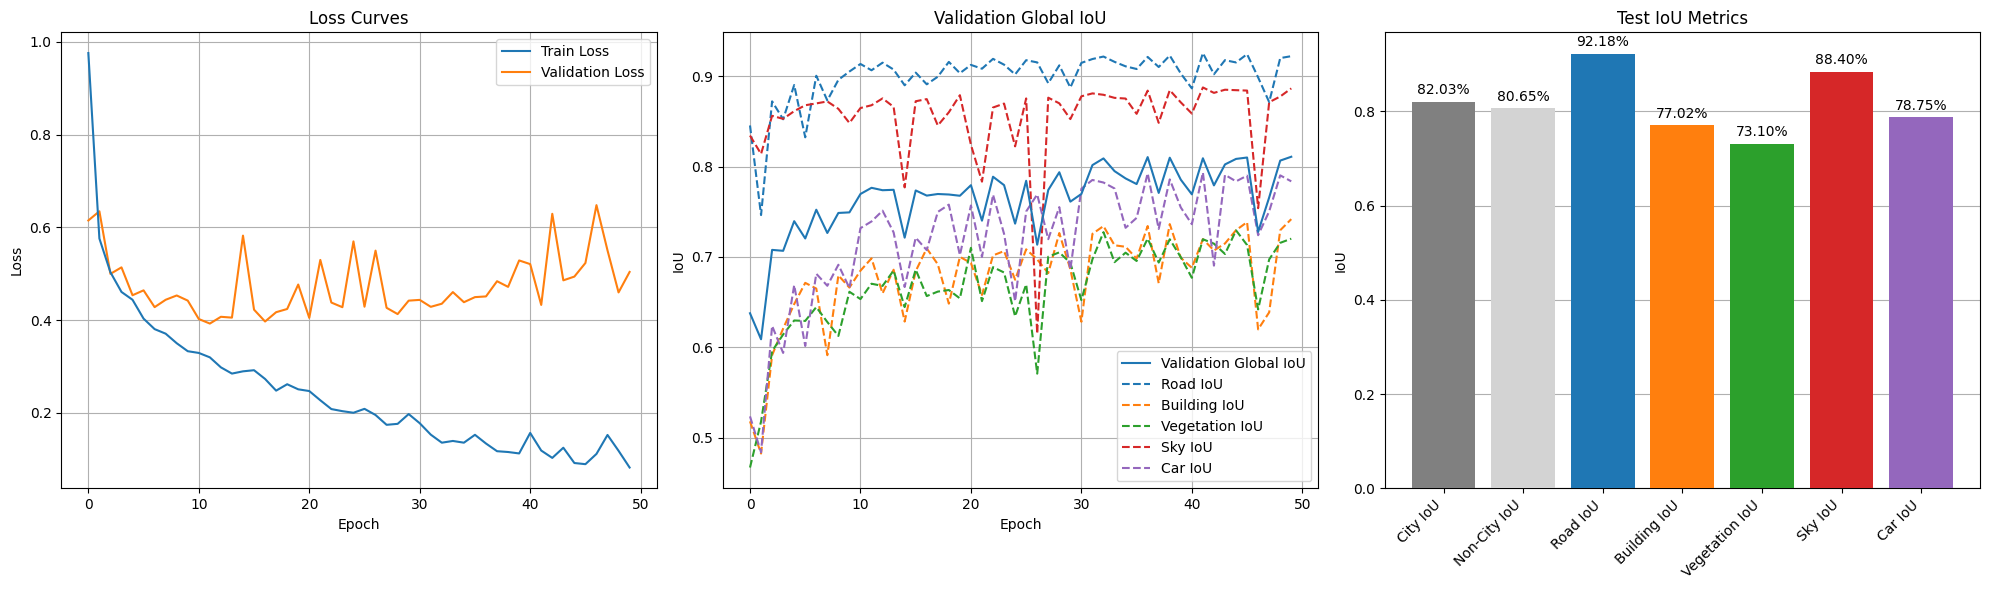
\includegraphics[width=0.6\textwidth]{figures/unet_overfit_training.png} 
    \caption{Training and Validation of the Vanilla U-Net with 128 Base Filters.}
    \label{fig:unet_overfit_training} 
\end{figure}

The experiment yielded the desired result of \textbf{overfitting}. Though the implemented trainer always saves the model at its \textbf{lowest validation loss}, thats where best generalization was reached.

\subsection{Sampled Results}

\begin{figure}[h] 
    \centering 
    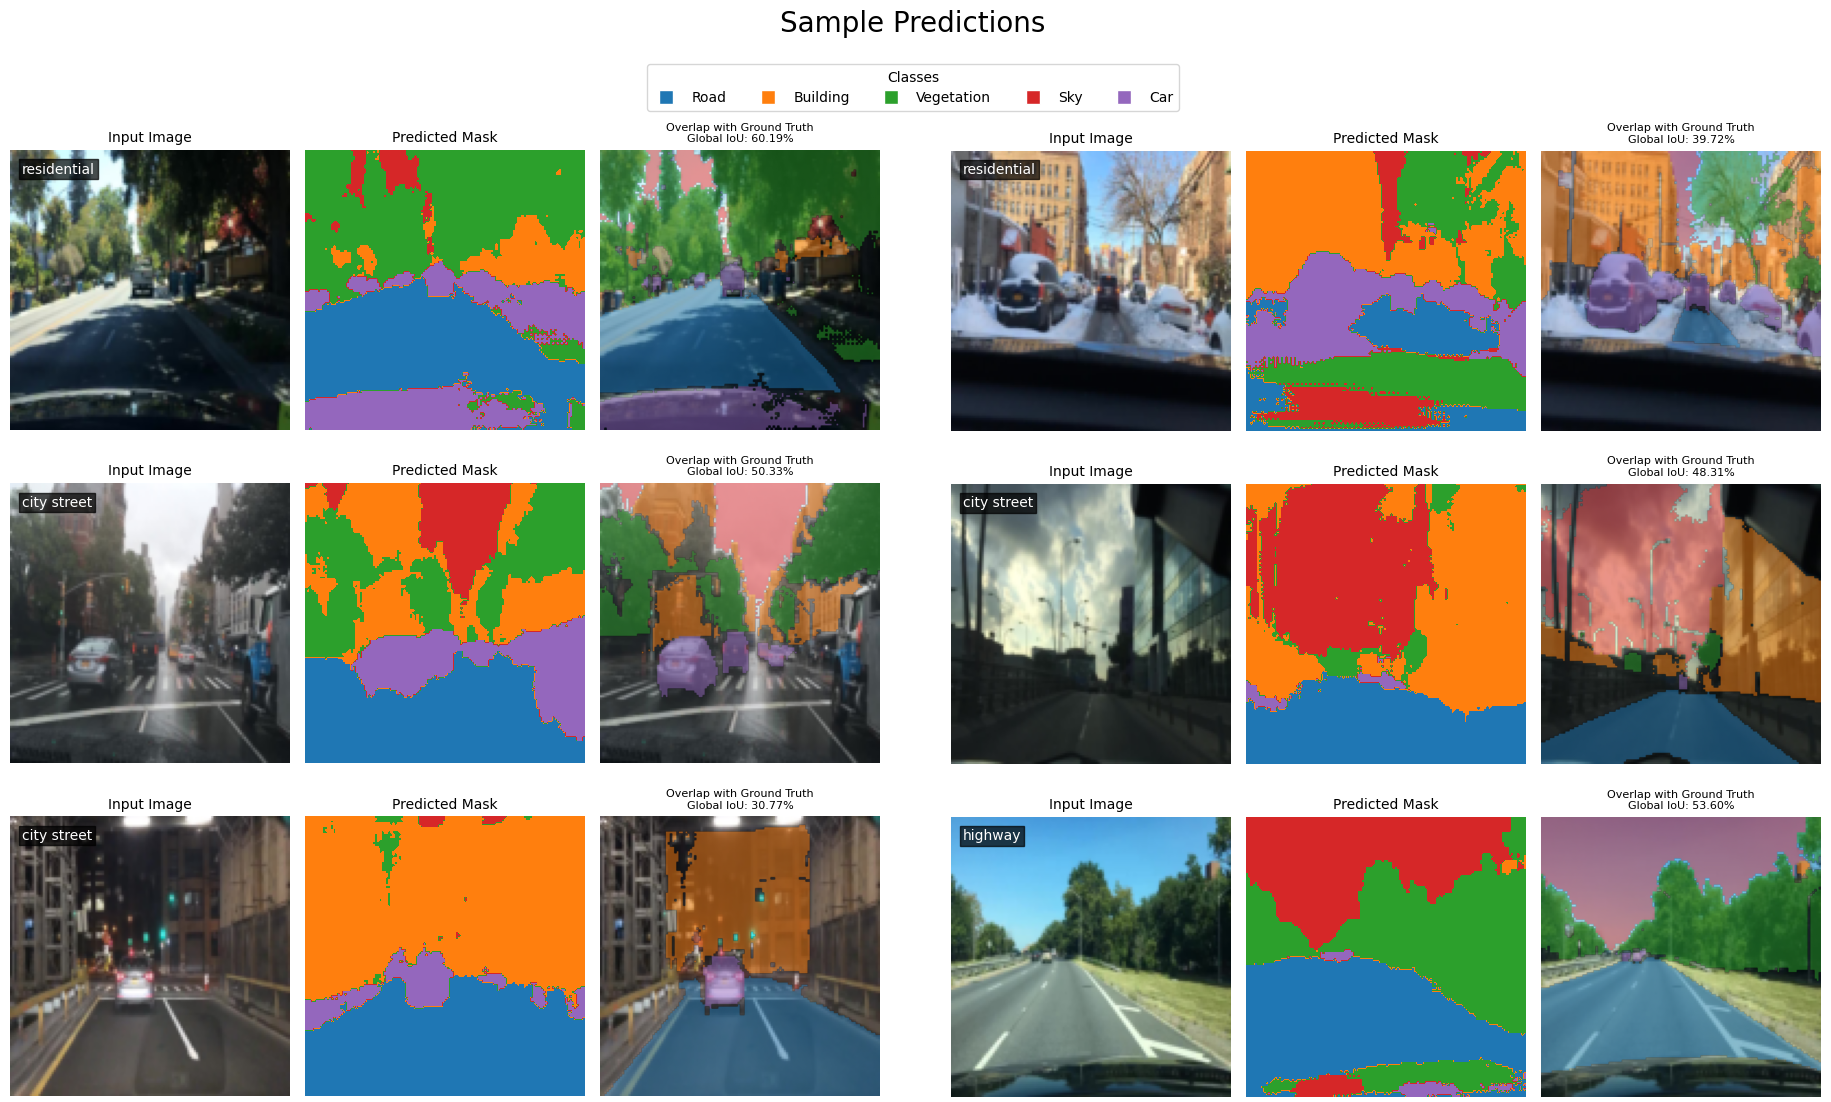
\includegraphics[width=0.6\textwidth]{figures/overfit_samples.png} 
    \caption{Difficult Samples predicted by the Vanilla U-Net}
    \label{fig:overfit_samples} 
\end{figure}

The rather simple Vanilla U-Net also performs surprisingly well when taking a visual inspection at the results of some difficult samples. Both the \texttt{road} and \texttt{car} classes are predicted well. There are some samples where the model seems to struggle, for example in snowy scenes where the road is not entirely visible. 

\section{Attention U-Net}

The Attention U-Net essentially is a Vanilla U-Net but with Attention Blocks built in. In the beginning experiments with the Attention U-Net I observed that it did started to overfit quite quickly due to the added parameters. This is when I decided to explore adding dropout and found a dropout rate of 20\% to be beneficial.

\subsection{Training}

\begin{figure}[h] 
    \centering 
    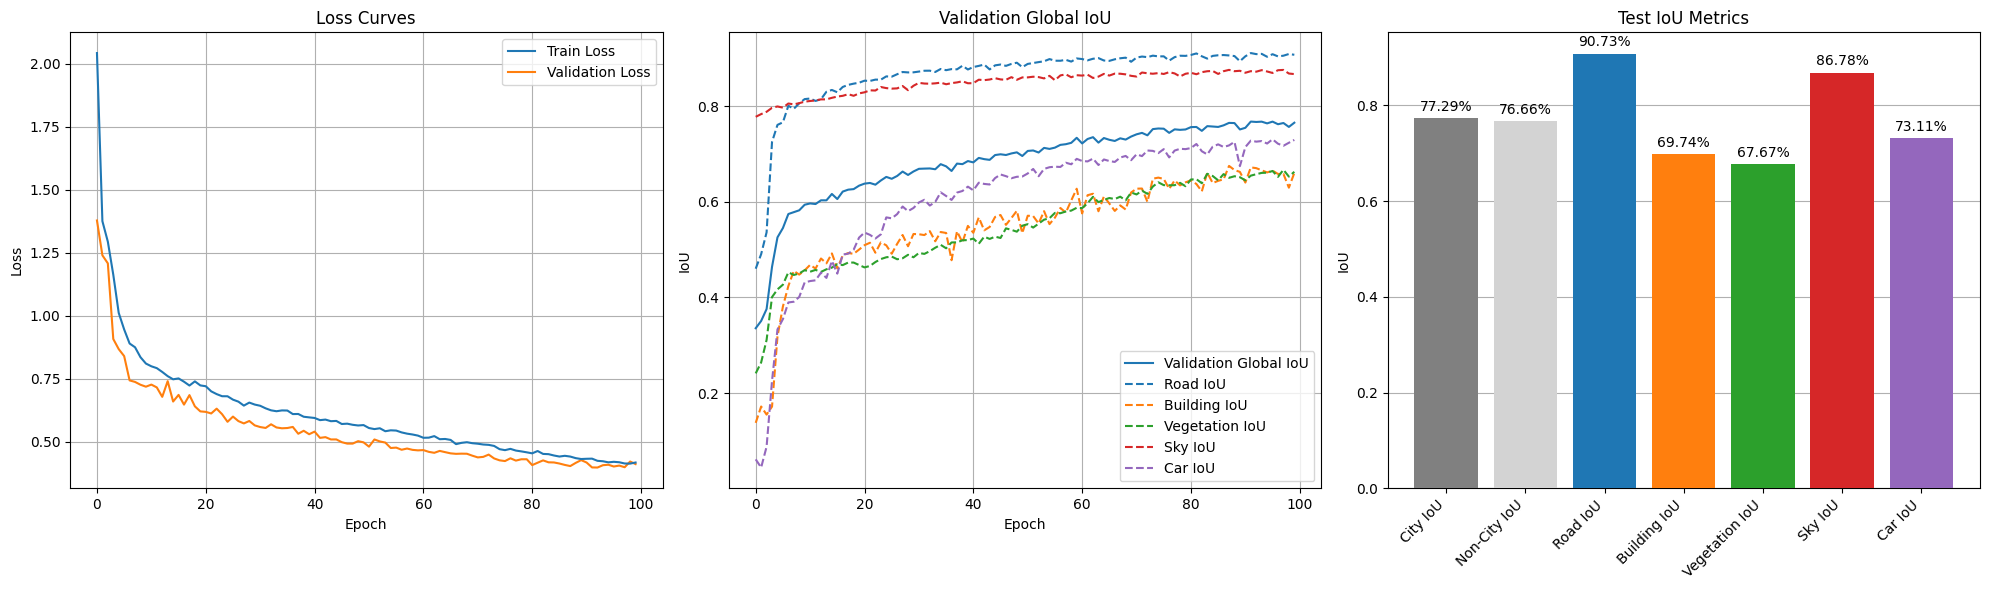
\includegraphics[width=0.6\textwidth]{figures/attention_dropout_training.png} 
    \caption{Training and Validation of the Attention U-Net with Dropout.}
    \label{fig:attention_dropout_training} 
\end{figure}

Contrary to the Vanilla U-Net's loss curves we can now observe in the Attention U-Net that the validation loss is decreasing along with the training loss. This is a good sign that the model is not overfitting and starting to generalize well since the validation loss starts to converge.

\subsection{Sampled Results}

\begin{figure}[h] 
    \centering 
    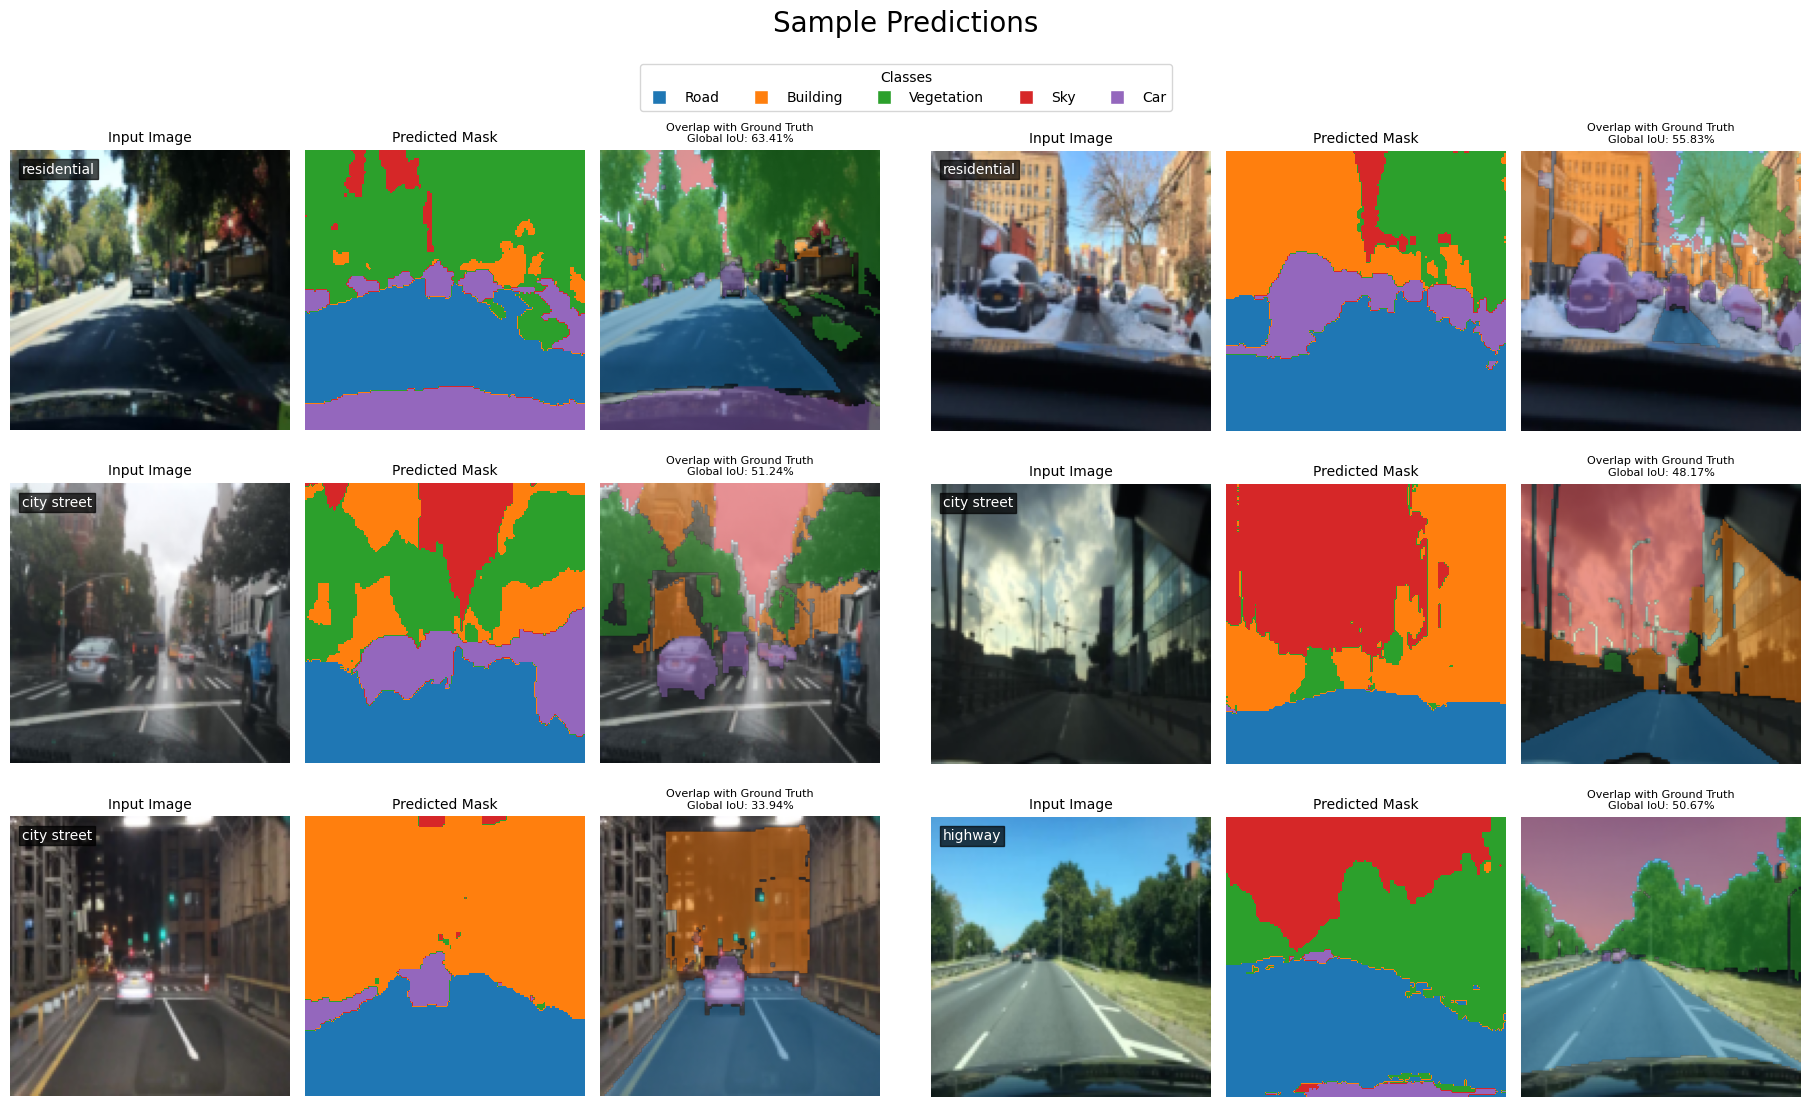
\includegraphics[width=0.6\textwidth]{figures/attention_samples.png} 
    \caption{Difficult Samples predicted by the Attention U-Net}
    \label{fig:attention_samples} 
\end{figure}

Even though the numerical metrics of the Vanilla U-Net are slightly better, the Attention U-Net seems to perfomr better in the samples where the best Vanilla U-Net still had some difficulties. For example, in the first sample, the Attention U-Net gets an even better understanding of smaller segments and labels that lie in the shadow. This is also observable in the fourth sample where the road is covered in snow.

\clearpage
\subsection{Saliency Maps}
As a last step in the Attention Mechanism exploration I also wanted to look at the saliency maps of the attention mechanism.

\begin{figure}[H] 
    \centering 
    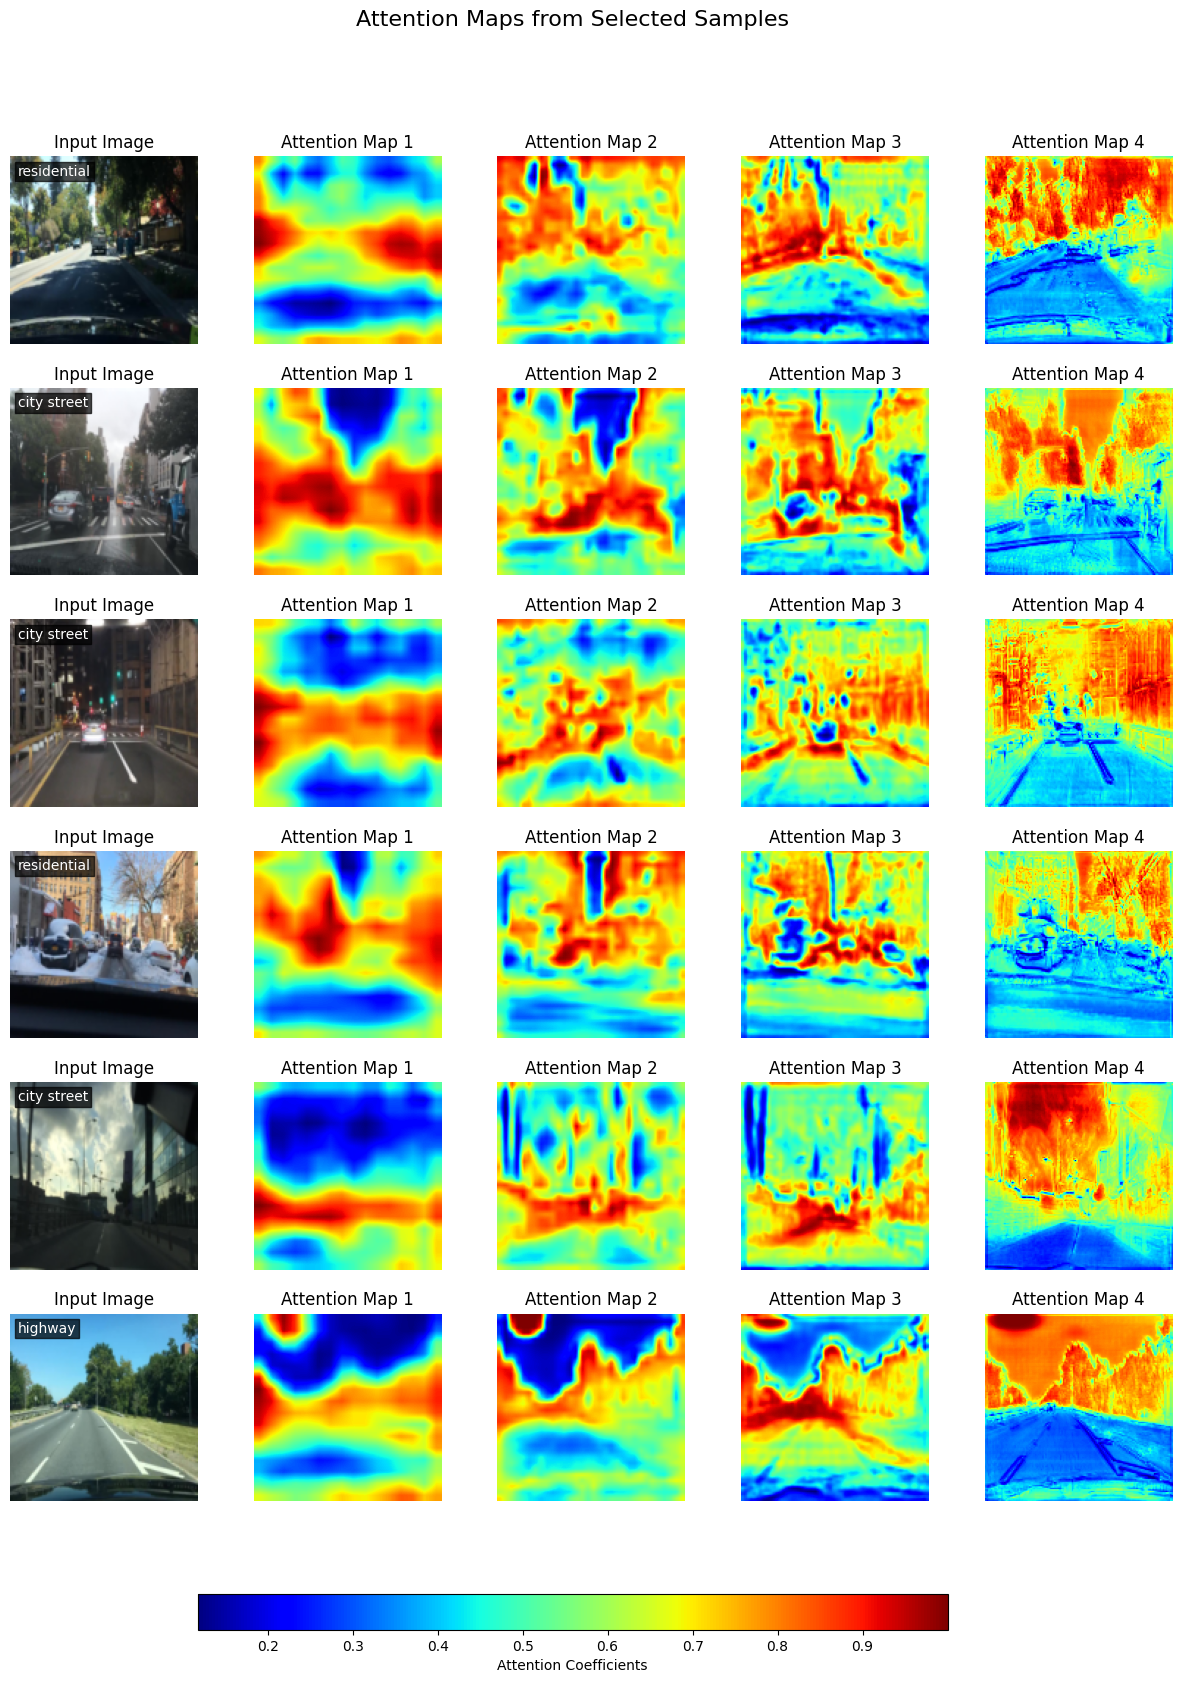
\includegraphics[width=0.5\textwidth]{figures/saliency_maps.png} 
    \caption{Saliency Maps of the Attention Mechanisms $\psi$ Coefficient.}
    \label{fig:saliency_maps} 
\end{figure}

The first attention layer seems to focus on the general location of the objects, it especially attends to the sides of the streets. This could be due to the fact that often times the sides are the biggest discriminator for what will be in a scene. For example, in the second sample, the image has a lot of different objects. The attention layer at that point attends to all objects on the sides where compared with the last sample, the attention layer does not have too many objects that are "hard to classify" as the scene is mostly just \texttt{road} and \texttt{sky}. Though at this last sample, there is an interesting activation happening at the top left of the image - I can't really make out why that is but perhaps it gets some information from the image having clear skies at this point.

The second layer goes more into detail and focuses on clearer shapes, this is a pattern that can be observed in the following attention maps as well. At attention map 4 we can see the mechanism has clear shapes to attend on. The $\psi$ coefficient seems to be especially high for parts of the image with a lot of structure as that is where it can gather a lot of information for labeling.
